\noindent \textred{4.}
For the binary search tree (BST) in pre-order as \{8, 4, 16, 9, 19, 17, 22\}. \textbf{Please first draw the BST}, then show the result of following operations (each operation is carried out on the result of the previous
operation):
\begin{figure}[!h]
    \centering
    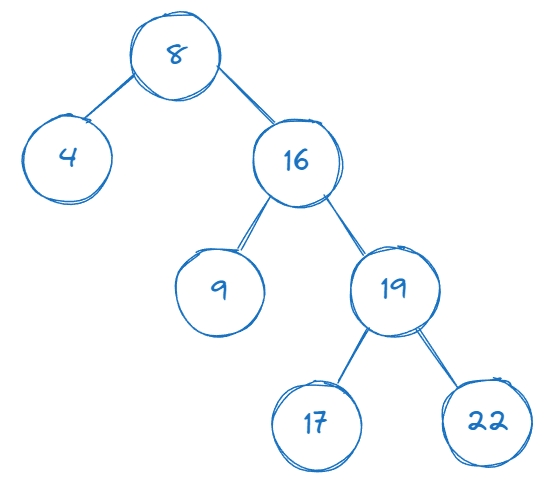
\includegraphics[width=0.4\linewidth]{HWs/HW6/figures/4-1.png}
    % \caption{Original BST}
    % \label{fig:bst-4}
\end{figure}

\noindent \begin{minipage}{0.5\textwidth}
(a) Insert key 20;
\begin{figure}[H]
    \centering
    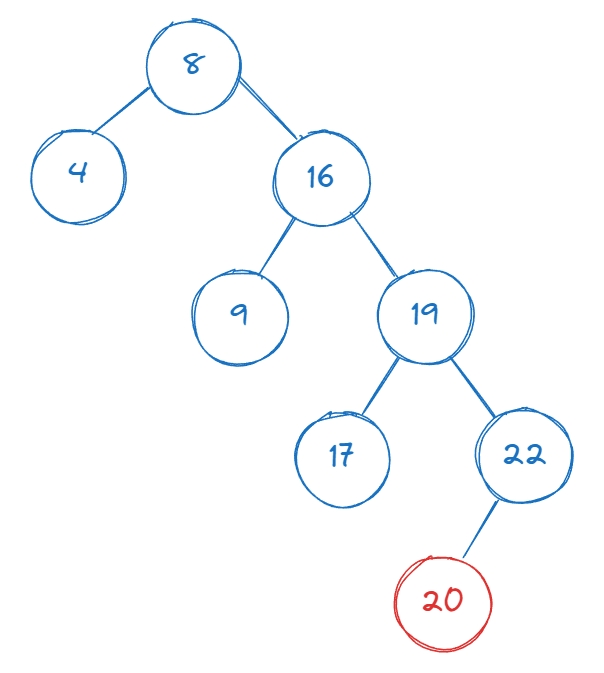
\includegraphics[width=0.8\linewidth]{HWs/HW6/figures/4-2.png}
\end{figure}
\end{minipage}
\begin{minipage}{0.5\textwidth}
(b) Then, delete key 8;
\begin{figure}[H]
    \centering
    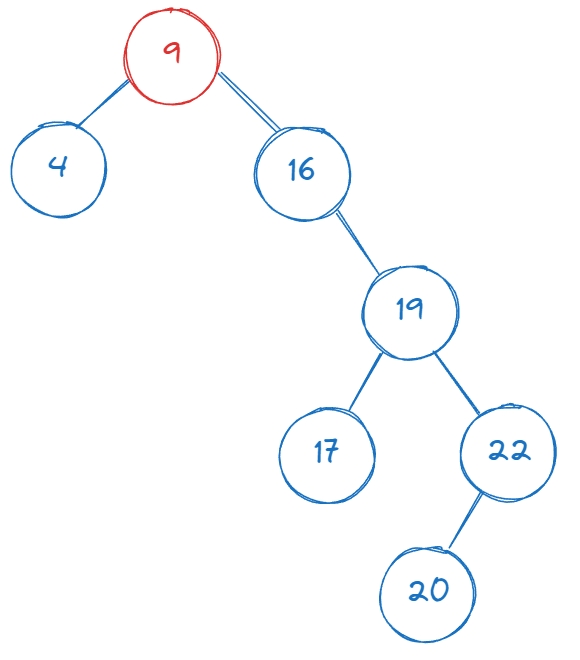
\includegraphics[width=0.8\linewidth]{HWs/HW6/figures/4-3.png}
\end{figure}
\end{minipage}

\vspace{10pt}
\noindent \begin{minipage}{0.5\textwidth}
(c) Then, delete key 19;
\begin{figure}[H]
    \centering
    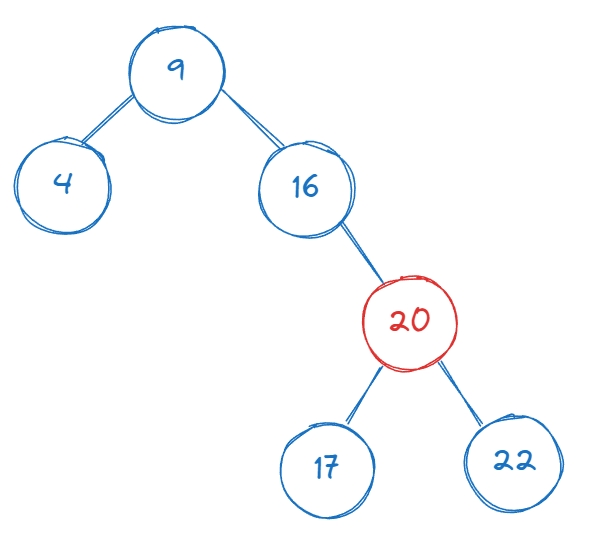
\includegraphics[width=0.8\linewidth]{HWs/HW6/figures/4-4.png}
\end{figure}
\end{minipage}
\begin{minipage}{0.5\textwidth}
(d) Finally, delete key 16.
\begin{figure}[H]
    \centering
    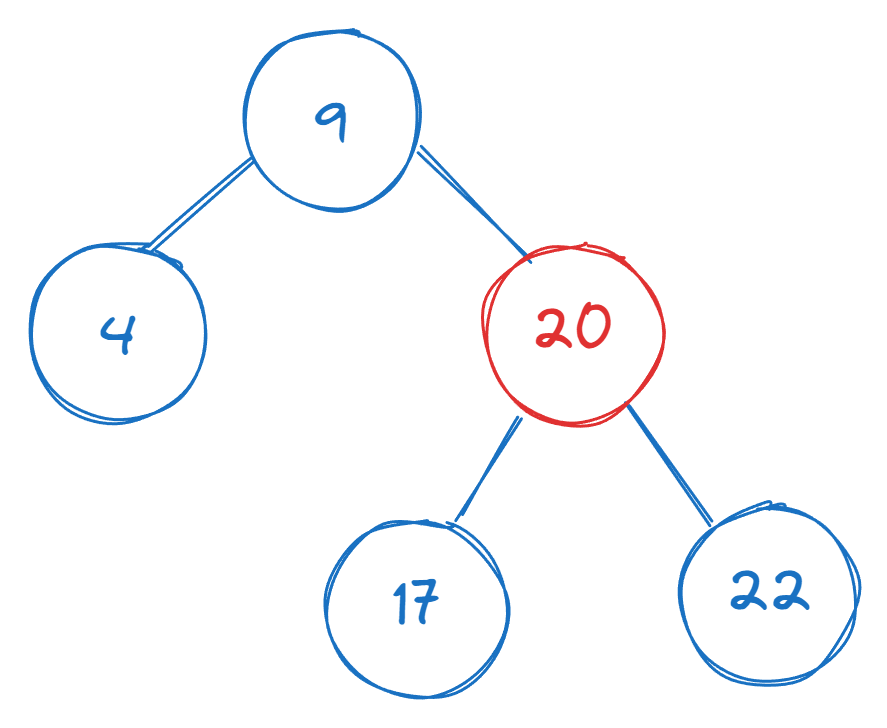
\includegraphics[width=0.6\linewidth]{HWs/HW6/figures/4-5.png}
\end{figure}
\end{minipage}



% \begin{enumerate}
%     \item[(a)] Insert key 20;
% \begin{figure}[!h]
%     \centering
%     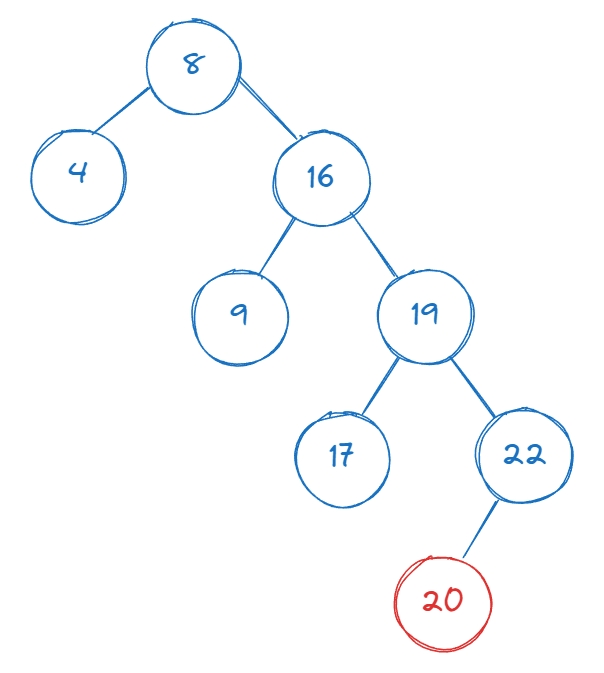
\includegraphics[width=0.3\linewidth]{HWs/HW6/figures/4-2.png}
% \end{figure}
%     \item[(b)] ss
% \begin{figure}[!h]
%     \centering
%     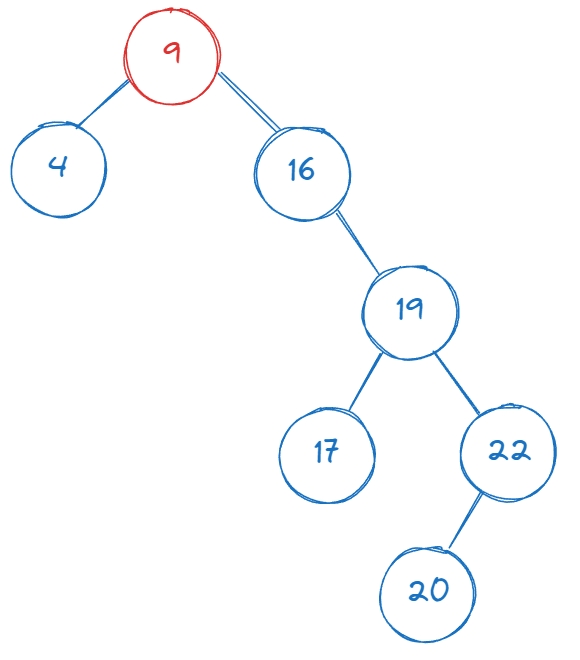
\includegraphics[width=0.3\linewidth]{HWs/HW6/figures/4-3.png}
% \end{figure}
%     \item[(c)] 
% \begin{figure}[!h]
%     \centering
%     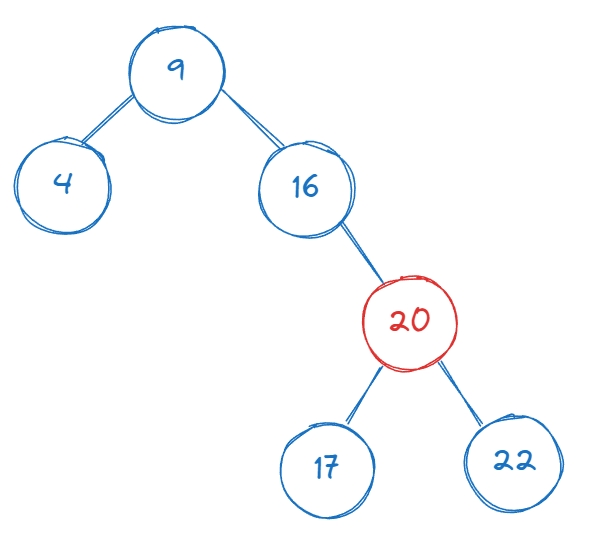
\includegraphics[width=0.3\linewidth]{HWs/HW6/figures/4-4.png}
% \end{figure}
%     \item[(d)] 
% \begin{figure}[!h]
%     \centering
%     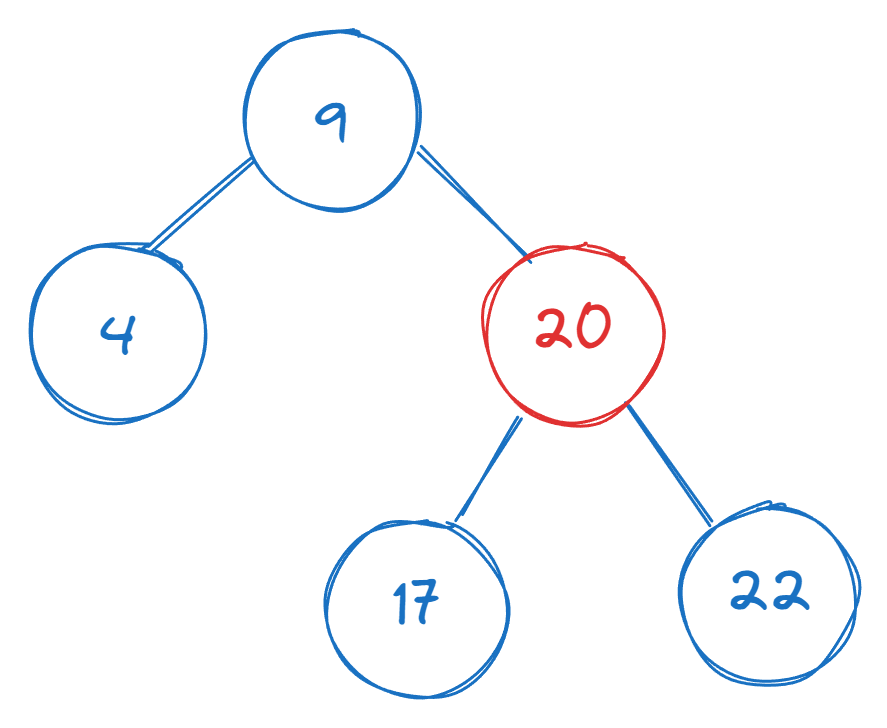
\includegraphics[width=0.3\linewidth]{HWs/HW6/figures/4-5.png}
% \end{figure}
% \end{enumerate}
